\documentclass[12pt, a4paper, oneside]{article} 
% velikost písma, stránky, typ dokumentu -- detaily viz literatura

\usepackage{czech} % nastavení češtiny
%\usepackage[latin2]{inputenc}
%\usepackage[cp1250]{inputenc} % pro win1250
\usepackage[center]{caption} 
\usepackage[utf8]{inputenc}
\usepackage{wrapfig} % nastavení obtékání textu
\usepackage{graphicx,amsmath} % nastavení grafiky, matematiky
\usepackage{subfig} % více obrázků vedle sebe 
\usepackage{float}
\usepackage{amsmath}
\usepackage{amssymb}
\usepackage{bbding}
\usepackage{enumitem}
\usepackage{breakurl}
\usepackage{pdflscape}
%\usepackage{indentfirst}

\usepackage{tocloft} %přidá tečky do obsahu ke kapitolám /sekcím 
\renewcommand{\cftsecdotsep}{\cftdotsep}

\usepackage[bookmarksopen,colorlinks,plainpages=false,linkcolor=black,urlcolor=blue,citecolor=black,filecolor=black,menucolor=black,unicode=true]{hyperref}

\urlstyle{rm}
%bookmarksopen -- open up bookmark tree 
%colorlinks -- zbarví odkazy (implicitně orámovaný nezbarvený text)
%urlcolor -- barva odkazů (implicitně magenta) 
%linkcolor=black -- barva odkazů v obsahu (implicitně red)

\usepackage{listings}
\usepackage{color}
\definecolor{lightgray}{RGB}{240,240,240}
\definecolor{darkgray}{rgb}{.4,.4,.4}
\definecolor{purple}{rgb}{0.65, 0.12, 0.82}
\definecolor{darkgreen}{RGB}{0,150,0}

\lstdefinelanguage{JavaScript}{
  keywords={typeof, new, true, false, catch, function, return, null, catch, switch, var, if, in, while, do, else, case, break, for},
  keywordstyle=\color{blue}\bfseries,
  ndkeywords={class, export, boolean, throw, implements, import, this},
  ndkeywordstyle=\color{blue}\bfseries,
  identifierstyle=\color{black},
  sensitive=zr,
  comment=[l]{//},
  morecomment=[s]{/*}{*/},
  commentstyle=\color{darkgreen}\ttfamily,
  stringstyle=\color{red}\ttfamily,
  morestring=[b]',
  morestring=[b]"
}

\lstset{
   backgroundcolor=\color{lightgray},
   extendedchars=true,
   basicstyle=\footnotesize\ttfamily,
   showstringspaces=false,
   showspaces=false,
   numbers=left,
   numberstyle=\footnotesize,
   numbersep=9pt,
   tabsize=2,
   breaklines=true,
   showtabs=false,
   aboveskip=5mm,
   belowskip=7mm,
   captionpos=b
}

\renewcommand{\listingscaption}{Příklad}
\renewcommand{\listoflistingscaption}{Příklady}

% \usepackage{parskip} -- zapne americké odstavce v celé práci

\addtolength{\textwidth}{-2mm} 
\addtolength{\hoffset}{4mm}  % posun textu kvůli kroužkové vazbě  

\setlength{\intextsep}{5mm} % nastavení mezery okolo obrázků

% nastavení příkazu >\figcaption pro popis čehokoli, jako by to byly obrázky 
\makeatletter   
\newcommand\figcaption{\def\@captype{figure}\caption}
\makeatother

\renewcommand\refname{Literatura} 
%\def\bibname{PŘÍLOHA D: Reference}
%\renewcommand\bibname{PŘÍLOHA D: Reference}
% přejmenuje anglický název Reference na české Literatura


%\makeindex % příprava pro výrobu indexu (jestli ho chcete)

%%    VLNKA <fileinput>  KkSsVvZzOoUuAaIi        
% Defaultni  koncovka pro <fileinput> je  ".tex"
%FIXME: haze error
%\cstieon % Vypne chovani vlnky jako tvrde mezery v matematickem rezimu

%%%%%%%%%%%%%%%%%%%%%%%%%%%%%%%%%%%%%%%%%%%%%%%%%%%%%%%%%%%%%%%
%V PROSTŘEDÍ ROVNIC SE NESMÍ VYSKYTOVAT PRÁZDNÝ ŘÁDEK
%
%PROGRAMY VLNKA A CSINDEX SE MUSÍ SPUSTIT SAMOSTATNĚ
%%%%%%%%%%%%%%%%%%%%%%%%%%%%%%%%%%%%%%%%%%%%%%%%%%%%%%%%%%%%%%%

% definice příkazů 
\newcommand{\D}{\medskip \noindent} % nový odstavec v "americkém" formátování 
\newcommand{\B}{\textbf} %tučné písmo
\newcommand{\A}{\mathbf} %tučné písmo v matematickém režimu
\newcommand{\TO}{\ensuremath{\boldsymbol\Omega}} % tučný znak velké omega -- pro ohmy
\newcommand{\I}{\index}  % vytváří položku indexu (asi nepoužijete)
\newcommand{\Deg}[1][]{\ensuremath{{#1}^\circ}} % vysází značku stupně Celsia
\newcommand{\Def}{\footnotesize Definice: \normalsize}
\newcommand{\Pos}{\footnotesize Experiment: \normalsize}
\newcommand{\Odv}{\footnotesize Odvození: \normalsize}
\newcommand{\Vym}{\footnotesize Vymezení pojmu: \normalsize}
\newcommand{\Ob}{obrázek }
\newcommand{\It}{\textit}  % kurzíva
\newcommand{\M}{\mathrm}   % v prostředí rovnic nastaví normální písmo (místo kurzívy ) 
\newcommand{\F}{\footnotesize} % zmenšená velikost písma
\newcommand{\N}{\normalsize} % normální velikost písma
%\newcommand{\U}{\underline}  % podtržené písmo
\newcommand{\e}{\ensuremath} 
\newcommand{\Has}{\textcolor{green}{\CheckmarkBold}}
\newcommand{\NoHas}{\textcolor{red}{\XSolidBrush}}
% další příkaz se aplikuje, pouze, když jste v matematickém režimu

%\hyphenation{Pusť-me pla-tí hod-no-ty do-sa-dí-me za-da-né dal-ším}
% dělení slov, kdyby implicitní nevyhovovalo

\linespread{1.3} 
% řádkování 1,5x  
% použijete podle situace  

\unitlength=1mm % nastavení volby jednotek 

% konec hlavičky
%%%%%%%%%%%%%%%%%%%%%%%%%%%%%%%%%%%%%%%%%%%%%%%%%%%%%%%%%%%%%%%%%%%
%%%%%%%%%%%%%%%%%%%%%%%%%%%%%%%%%%%%%%%%%%%%%%%%%%%%%%%%%%%%%%%%%%%


\begin{document}
\setlength{\voffset}{-20mm}
\begin{center}

\Large
\B{LORRIS TOOLBOX \\ Sada nástrojů pro vývoj a~řízení robotů}


\large
\url{http://tasssadar.github.io/Lorris}

Vojtěch Boček

\end{center}

\section*{Abstrakt}
Lorris Toolbox je komplexní sada nástrojů pro vývoj, ovládání a ladění libovolného zařízení schopného komunikovat po sériové lince nebo TCP socketu. Toto zahrnuje velkou část mikročipů používaných nejen v robotech všeho druhu, ale i v běžné spotřební elektronice.

Hlavním úkolem tohoto softwarového balíku je parsování a přehledné grafické zobrazení binárních dat, které zařízení posílá. K tomu slouží nástroj \B{analyzér}, který k zobrazení používá tzv. \It{widgety} -- malá okna, která zobrazují vždy určitou část dat jako číslo, sloupcový bar nebo například graf. Celé prostředí analyzéru je skriptovatelné, což umožňuje zpracování prakticky jakéhokoliv typu příchozích dat.

Mezi další nástroje patří \B{programátor}, který slouží jako grafické rozhraní pro programování mnoha typů mikročipů nebo klasický textový \B{terminál}, jež je stále neocenitelnou pomůckou pro každého vývojáře aplikací pro mikročipy.

Lorris je unikátní nástroj pro elektroniky a programátory, jehož hlavním přínosem je, že urychluje, zpřehledňuje a~hlavně výrazně zjednodušuje vývoj a~testování aplikací pro mikročipy, typicky programování a~řízení různých druhů robotů. Celá aplikace je na rozdíl od profesionálních nástrojů (kterým navíc často chybí potřebné funkce nebo mají velmi složité ovládání) \B{zdarma}, má \B{otevřený zdrojový kód} a běží jak pod operačním systémem MS Windows, tak pod Linuxem.

\newpage
\setlength{\voffset}{-10mm}
\section{Popis rozhraní}
Program je navrhnutý jako modulární aplikace, aby mohl zastřešit několik samostatných částí, které však mají podobnou oblast použití. Základní část programu poskytuje připojení k~zařízení (např. robot, deska s~čipem) a~ukládání nastavení aplikace, samotné zpracování dat probíhá v~modulech, které jsou otevírány v~panelech -- podobně jako stránky ve webovém prohlížeči. Lorris umí otevřít několik oken zaráz a~dokáže také rozdělit okno na několik částí, na obrázku \ref{split_img} je nalevo modul analyzér a~napravo terminál.

\begin{figure}[H]
\begin{center}
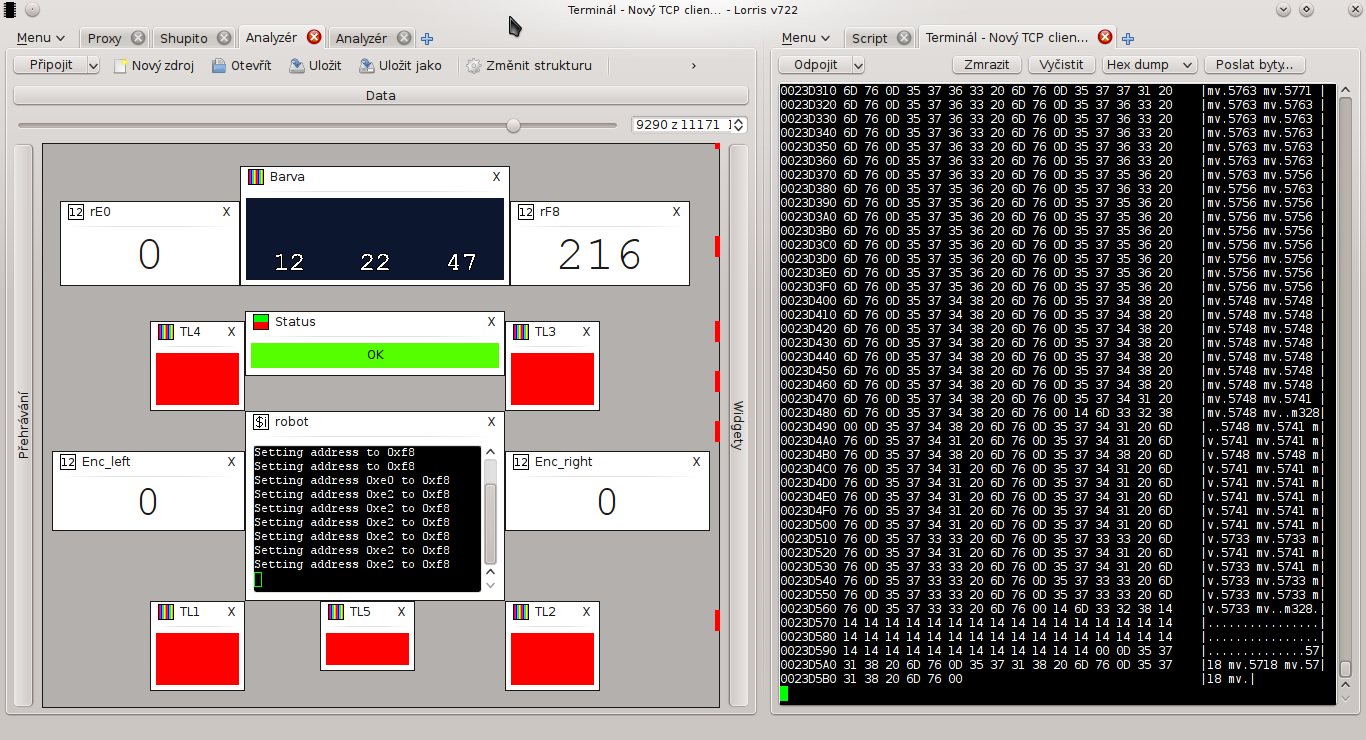
\includegraphics[width=\textwidth]{../img/split.png}
\caption{Ukázka rozdělení okna na více částí}
\label{split_img}
\end{center}
\end{figure}

\subsection{Sezení}
Lorris dokáže uložit vše, co má uživatel aktuálně otevřené (záložky, jejich uspořádání, informace o~připojení, data jednotlivých záložek atd.), jako tzv. sezení (anglicky \It{session}). Sezení je možné později načíst a~tímto se vrátit k~předchozí práci. Lorris automaticky ukládá sezení před svým ukončením, takže když uživatel program znovu otevře, vše je ve stejném stavu, jako když aplikaci opouštěl.

\newpage
\section{Modul: Analyzér}

\begin{figure}[h]
\begin{center}
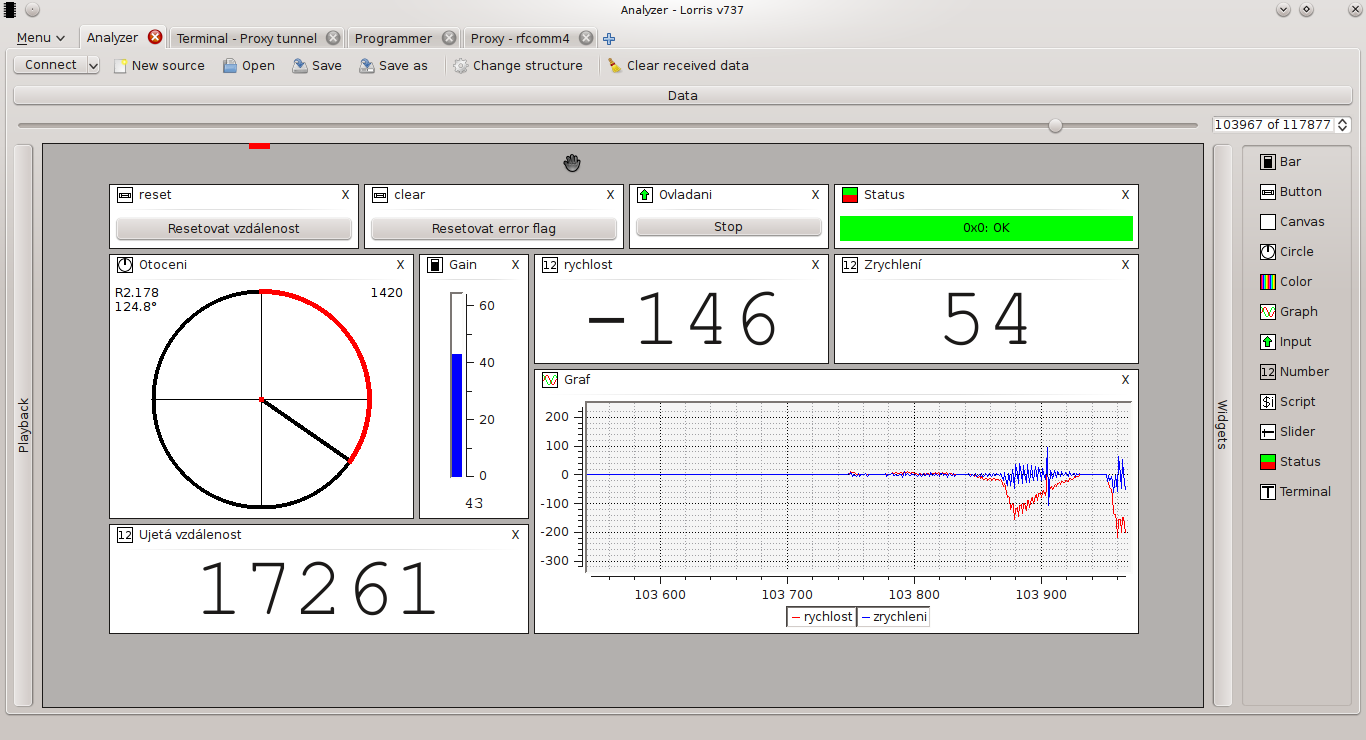
\includegraphics[width=\textwidth]{../img/analyzer_all.png}
\caption{Modul analyzér}
\label{Analyzer}
\end{center}
\end{figure}

Tento modul parsuje data (strukturované do packetů) přicházející ze zařízení a~zobrazuje je v~grafických \uv{widgetech}. Zpracovaná data si aplikace ukládá do paměti -- listování packety je možné pomocí posuvníku a~boxu v~horní části okna. Data (přijatá data, strukturu packetů a~rozestavení a~nastavení widgetů) je také možné uložit do souboru a~později zase v~programu otevřít.

Po nastavení struktury se přijatá data začnou po packetech zobrazovat v~horní části okna, a~v~pravé části se zobrazí sloupeček s~dostupnými zobrazovacími widgety. Widgety se dají pomocí drag\&drop principu \uv{vytahat} na plochu v~prostřední části okna. Data se k~widgetu přiřadí taktéž pomocí drag\&drop, tentokrát přetažení prvního bajtu dat na widget. 

Poté widget zobrazuje data tohoto bajtu, nebo tento bajt bere jako první, pokud jsou data delší. Aby bylo možné zpětně poznat, který bajt je k~widgetu přiřazen, je po najetí myši na widget červeně zvýrazněn.

Nastavení widgetu jsou přístupná v~kontextovém menu po pravém kliknutí myší na widget. Nastavit lze jméno a~další parametry podle typu widgetu -- podrobněji jsou možnosti nastavení popsány u~jednotlivých widgetů. Widgety je taktéž možné \uv{uzamknout}, aby nebylo možné je zavřít, měnit jejich pozici a~velikost.

Widgety je možné přesně rozmisťovat pomocí \uv{přichytávání} k~síti anebo k~ostatním widgetům pomocí zarovnávacích čar. Lze je také jednoduše a~rychle duplikovat pomocí chycení a přetažení se stisknutou klávesou control -- místo přesunutí se widget zkopíruje a uživatel v té chvíli přesunuje jeho kopii.

U~některých widgetů se může hodit následující funkce: widgety je možné rychle zvětšit tak, aby zabraly celou viditelnou plochu pomocí jednoduchého  gesta myší~--~stačí widget chytit jako při přesouvání a~\uv{zatřepat} s~ním zleva doprava. Při opětovném přesunutí se pak widget zmenší na svoji původní velikost.
\\
\\
\noindent \B{Typy widgetů v analyzéru:}
\begin{itemize}
 \setlength{\itemsep}{1pt}
 \setlength{\parskip}{0pt}
 \setlength{\parsep}{0pt}
\item Sloupcový bar
\item Barva
\item Číslo
\item Graf
\item Kolo (zobrazení úhlu na kružnici)
\item Natočení (natočení objektu ve 3D prostoru)
\item Plátno (kreslení 2D grafiky)
\item Script
\item Slider
\item Status
\item Terminál
\item Tlačítko
\item Vstup (pro uživatelský vstup)
\end{itemize}

\section{Modul: Proxy mezi sériovým portem a~TCP socketem}
\begin{figure}[H]
\begin{center}
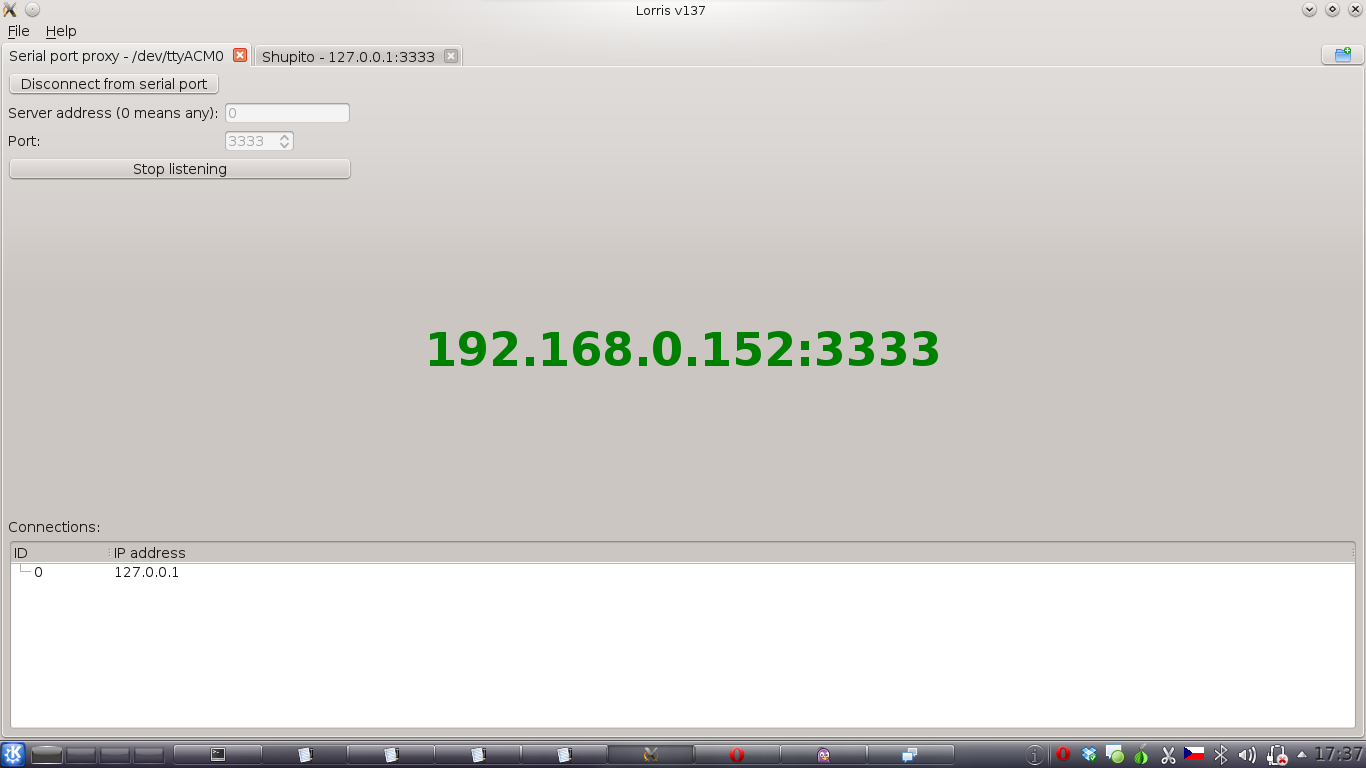
\includegraphics[width=\textwidth]{../img/proxy.png}
\caption{Proxy mezi sériovým portem a~TCP socketem}
\label{Shupito}
\end{center}
\end{figure}
Jednoduchá proxy mezi sériovým portem a~TCP socketem. Vytvoří server, na který je možné se připojit z~Lorris nebo jiného programu na jiném počítači. Po připojení se přeposílají data ze sériového portu připojeným klientům a~naopak.

V praxi to znamená, že je možné přes internet na dálku ovládat robota nebo nahrát program do čipu.

\newpage
\setlength{\voffset}{0mm} % posune text/obrázek na této stránce, kam patøí
\pagestyle{plain}

\section{Modul: Programátor}
\begin{figure}[H]
\begin{center}
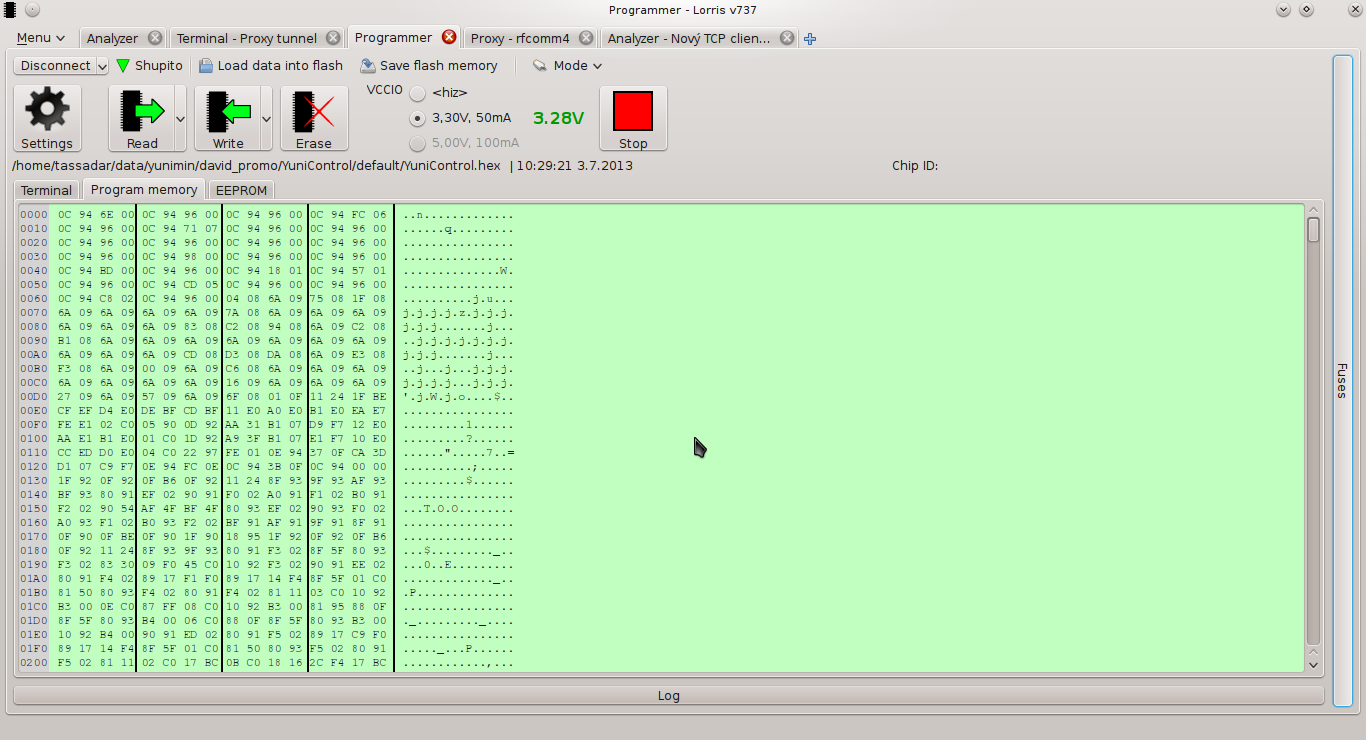
\includegraphics[width=\textwidth]{../img/programmer.png}
\caption{Modul Programátor}
\label{prog_full}
\end{center}
\end{figure}

%TODO: rozšířit
Tento modul funguje jako grafické rozhraní pro několik typů programátorů a~bootloaderů. Podporuje dva typy rozhraní -- plné (obrázek \ref{prog_full}) a~zmenšené (obrázek \ref{prog_mini}). Plné rozhraní obsahuje tlačítka a~nastavení pro programování všech pamětí čipu, zmenšené rozhraní pak obsahuje pouze tlačítko na programování hlavní paměti a~zastavení čipu. Zmenšený mód je vhodný při rozdělení okna na více částí protože obsahuje pouze nejpoužívanější prvky a~nezabírá zbytečně místo.

\begin{figure}[H]
\begin{center}
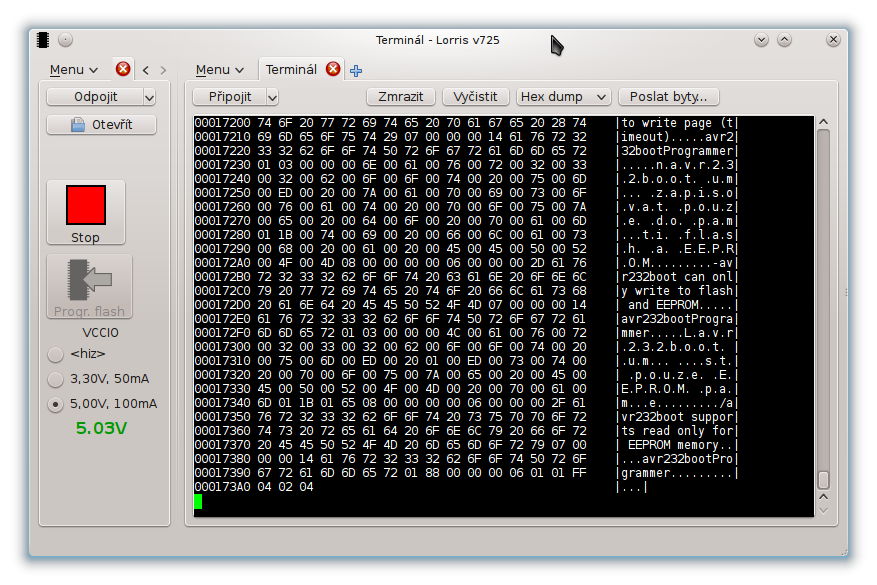
\includegraphics[width=\textwidth]{../img/programmer_mini.png}
\caption{Zmenšené UI modulu \It{programátor} (nalevo) s~otevřeným \It{terminálem}}
\label{prog_mini}
\end{center}
\end{figure}

\subsection{Programátor Shupito}
Shupito je programátor mikročipů vytvořený Martinem Vejnárem, který dokáže programovat mikrokontroléry pomocí ISP\footnote{\It{In-system programming} -- rozhraní, které umožňuje programovat čipy přímo na desce plošného spoje.}, PDI\footnote{\It{Program and Debug Interface} -- rozhraní firmy Atmel umožňující programování čipů přímo na desce, podobně jako ISP} a~JTAG\footnote{\It{Joint Test Action Group} -- rozhraní podle standardu IEEE 1149.1 umožňující mimo jiné programování a~debugování čipů} rozhraní. 

Modul programátor v~mojí práci slouží jako oficiální rozhraní pro Shupito. Převážná část komunikace s~programátorem je napsána samotným Martinem Vejnárem.

\newpage
\section{Modul: Terminál}
\begin{figure}[H]
\begin{center}
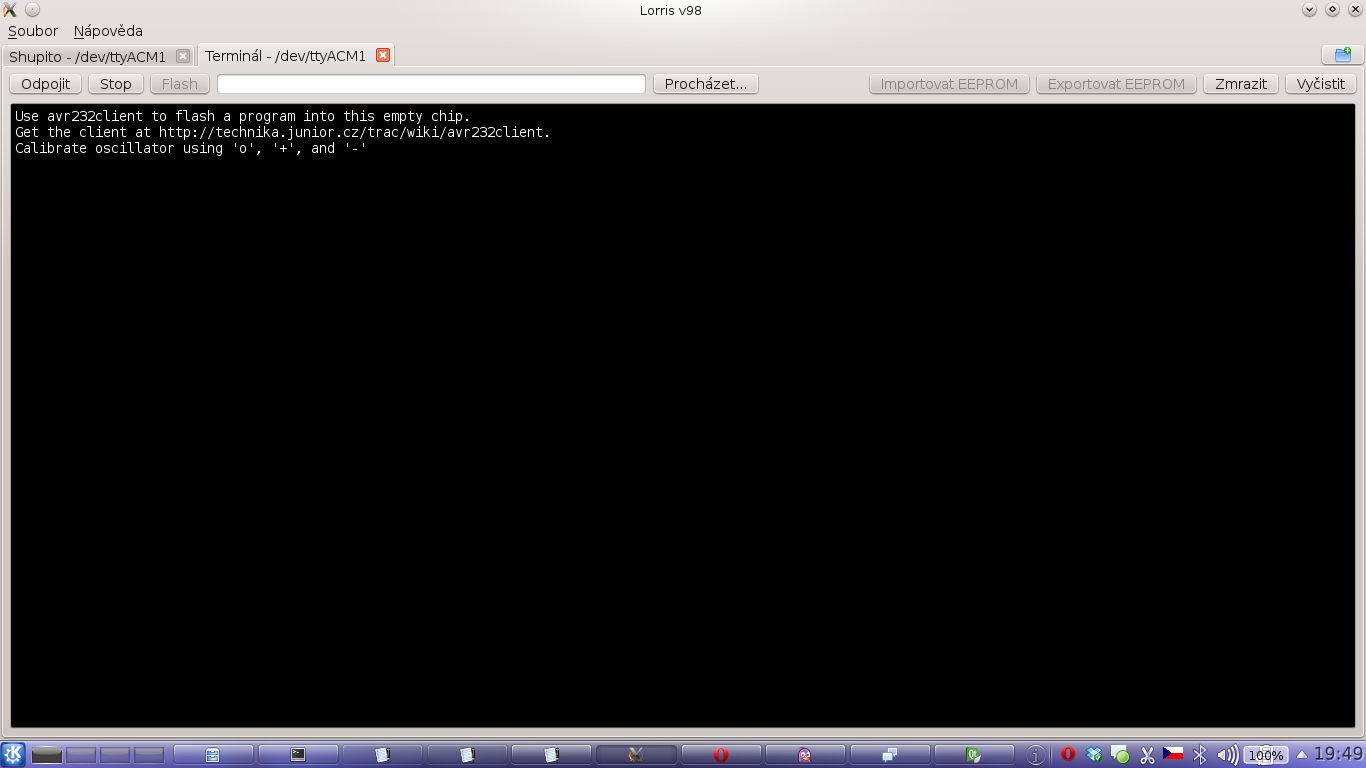
\includegraphics[width=\textwidth]{../img/terminal.png}
\caption{Modul terminál}
\label{Terminal}
\end{center}
\end{figure}
Základní pomůcka při práci s~mikrokontroléry, běžný textový terminál -- zobrazuje data přijatá přes sériový port a~posílá stisky kláves. Kromě klasického textového módu dokáže příchozí data zobrazovat jako hexadecimální hodnoty všech příchozích bajtů.

Terminálu je možné nastavit barevné schéma, velikost a~font textu, jaká sekvence kontrolních znaků se má odeslat při stisknutí klávesy enter a~chování některých kontrolních znaků (například jestli má znak \verb|\n| vytvořit nový řádek nebo ne).

\newpage
\section{Aplikace pro Android}
\begin{figure}[H]
\begin{center}
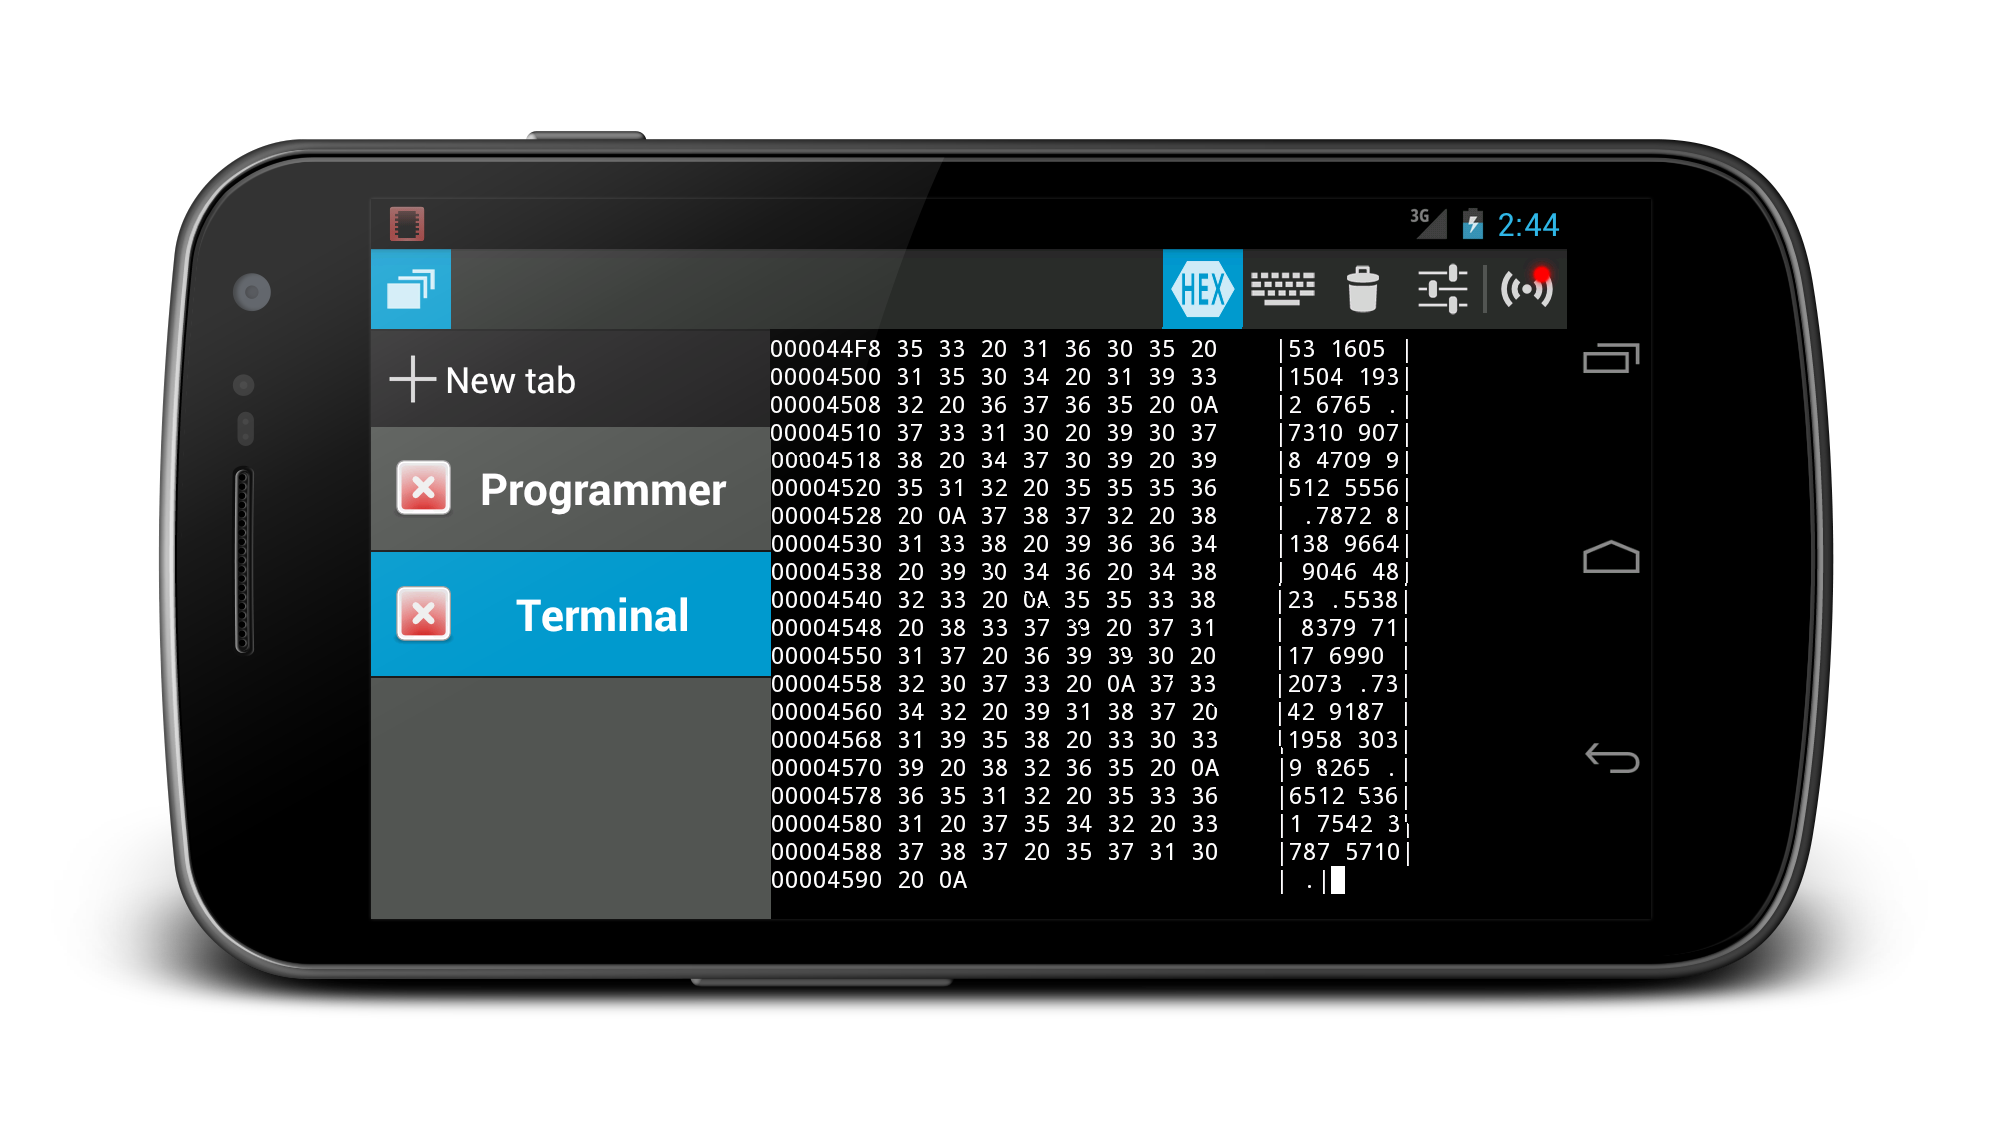
\includegraphics[width=\textwidth]{../img/mobile.png}
\caption{Lorris mobile}
\end{center}
\end{figure}
Jako další vývojový stupeň jsem začal s~vývojem Lorris pro platformu Google Android, protože chytrá zařízení s~tímto operačním systémem jsou často při ruce a~stačí k~rychlému vyřešení menšího problému.

Aplikace {\bf Lorris mobile} slouží jako přenosný doplněk k~počítačové verzi Lorris -- nemusí nutně obsahovat všechny funkce desktopové aplikace, ale má pomoci zejména když je v~terénu potřeba rychle něco přenastavit či poupravit.

Aplikace funguje na telefonech a~tabletech s~OS Android ve verzi 2.2 a~vyšší, je optimalizována i~pro větší obrazovky tabletů a~je dostupná v~oficiálním distribučním kanále Android aplikací -- v~obchodě Google Play, stačí hledat heslo \uv{Lorris}.

Lorris mobile má podobnou architekturu jako desktopová verze Lorris. Začíná se vytvořením sezení, do kterého se ukládá vše, co uživatel v~aplikaci otevře. Po vytvoření a~otevření sezení se uživatel dostane na hlavní obrazovku programu, kde si může otevřít jednotlivé moduly v~záložkách podobně jako v~desktopové aplikaci.

\subsection{Programátor}
\begin{figure}[H]
\begin{center}
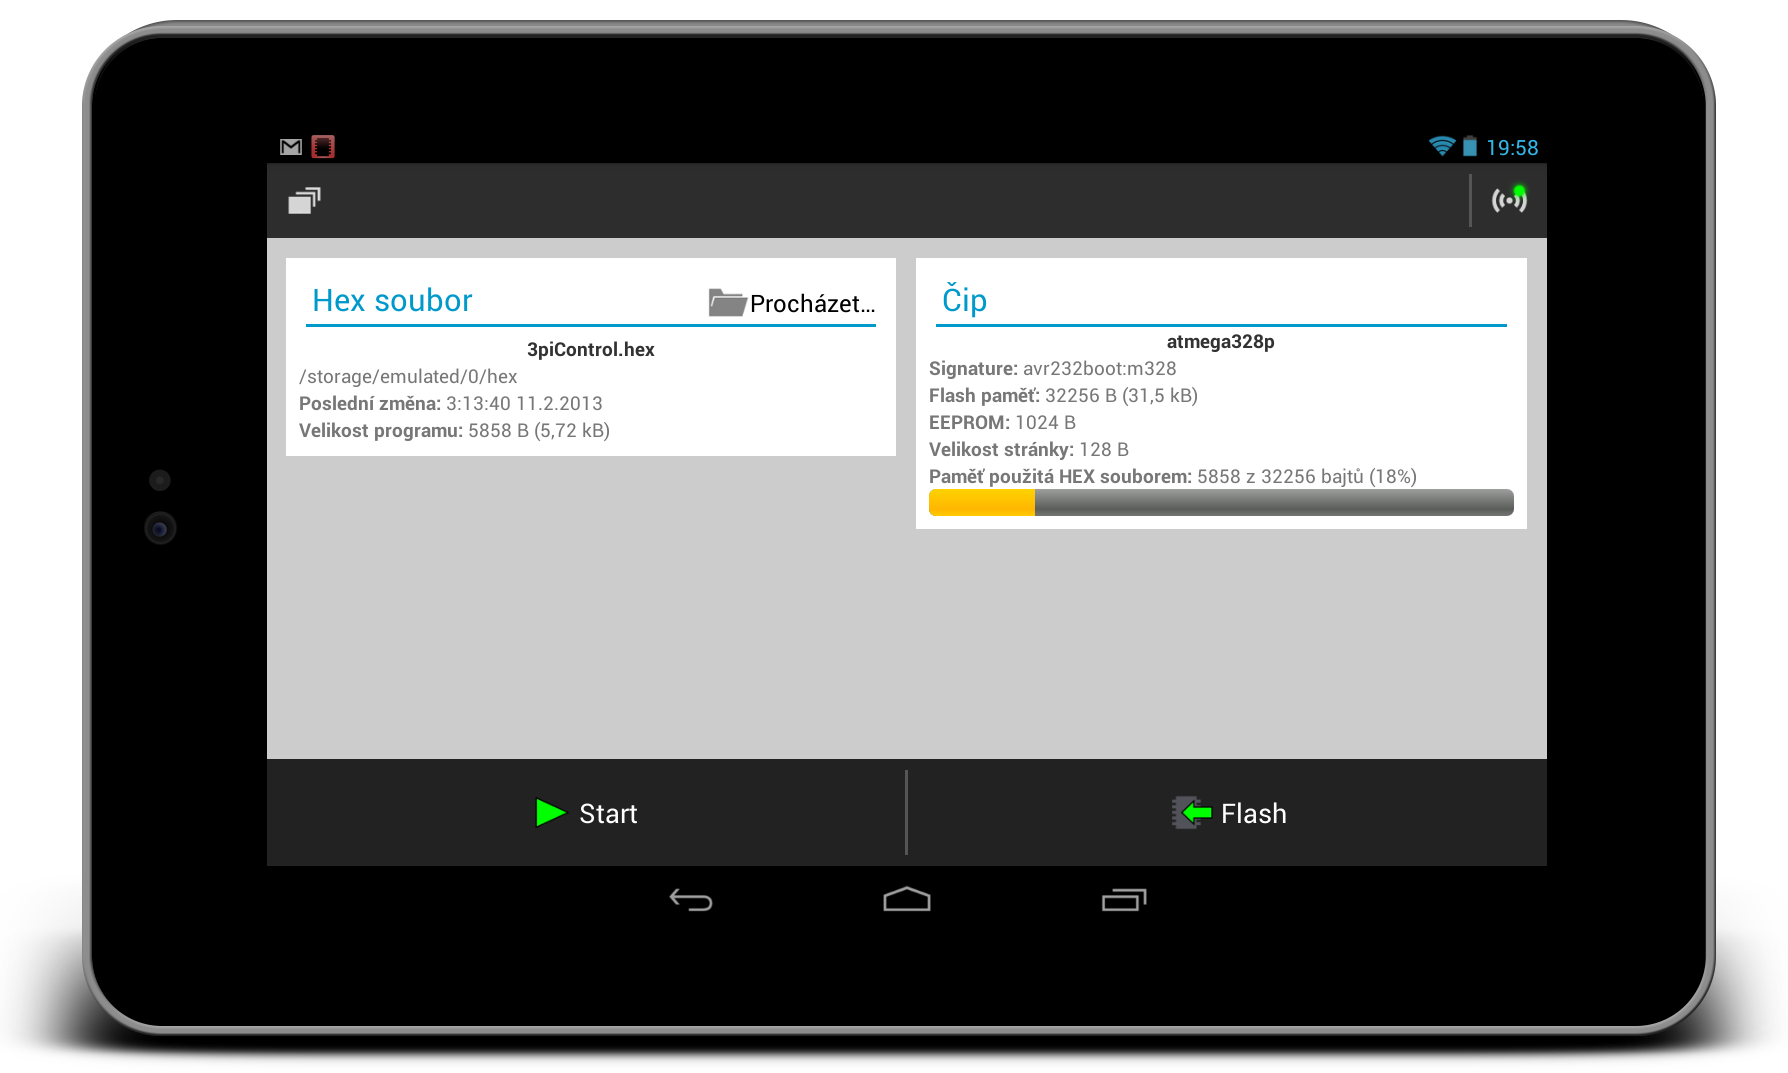
\includegraphics[width=\textwidth]{../img/mobile_programmer.png}
\caption{Lorris mobile -- programátor}
\end{center}
\end{figure}
Modul programátor dokáže programovat čipy pomocí bootloaderů {\bf avr232boot} a~{\bf AVROSP} a~také pomocí programátoru Shupito.
Tato část Lorris mobile používá části nativního kódu z~desktopové verze Lorris, díky tomu se kód lépe spravuje a~je rychlejší.

\subsection{Terminál}
\begin{figure}[H]
\begin{center}
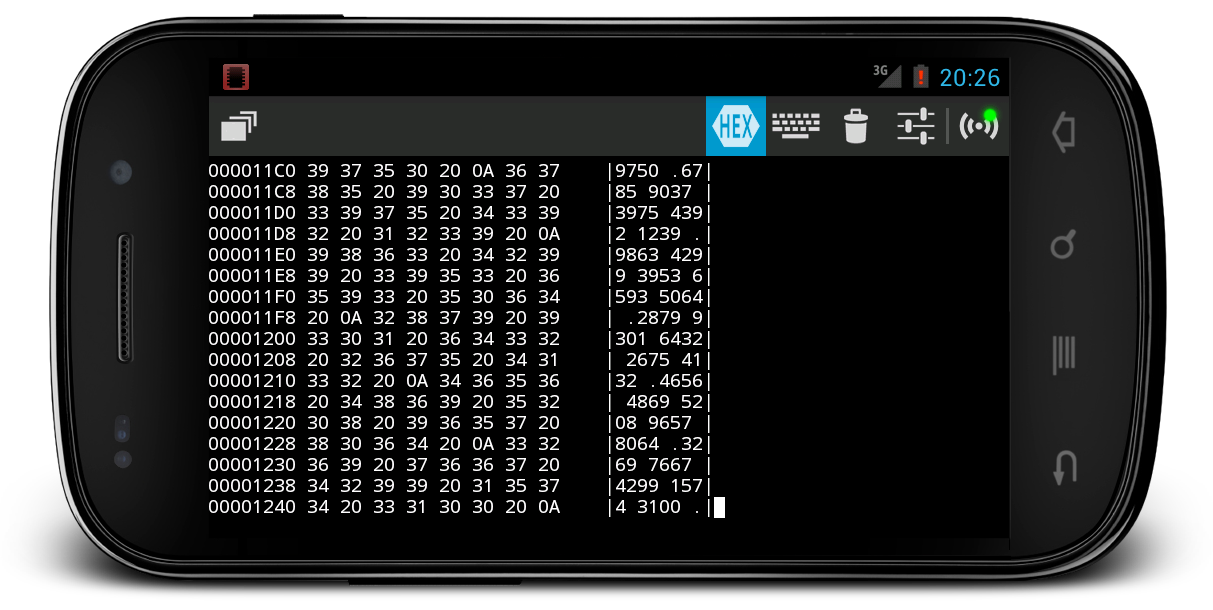
\includegraphics[width=\textwidth]{../img/mobile_term.png}
\caption{Lorris mobile -- terminál}
\end{center}
\end{figure}
Tento modul představuje běžný textový terminál. Umí většinu funkcí terminálu v~desktopové verzi Lorris -- zobrazuje data (jako text nebo hexadecimální hodnoty bajtů), odesílá stisky kláves, lze nastavit velikost a~barva textu, barvu pozadí a~jaké kontrolní znaky se mají odeslat při stisknutí klávesy enter. 


\newpage
\section{Reálné nasazení}
\label{usage}
\subsection{DDM Junior}
Prvními uživateli sady Lorris se stali od samého začátku vývoje před několika lety členové některých technicky zaměřených kroužků na DDM Junior v~Brně. Lorris zde pomáhá při stavbě různých zařízení, zejména robotů, a~žáci, kteří se učí programovat mikrokontroléry, používají programátor \It{Shupito} a~tím pádem i~modul Programátor z~balíku Lorris. V~průběhu výuky programování mikrokontrolérů pomáhá také modul Terminál (jednoduchá komunikace s~čipem) a~později i~Analyzér (pokročilé zpracovávání dat z~čipu).

Lorris je pro použití v~DDM Junior vhodná také díky nulové pořizovací ceně -- větší firma, zabývající se vývojem aplikací pro mikrokontroléry, by pravděpodobně pořídila drahý komerční program s~podobnými funkcemi jako má Lorris nebo vyvinula vlastní jednoúčelové aplikace. Pro příspěvkové organizace typu DDM je však řešení používané velkými firmami poněkud nedostupné.

K~dnešnímu dni má Lorris přibližně 20 uživatelů jen z~řad DDM Junior. Díky postupnému rozšiřování programátoru \It{Shupito} mezi uživatele po celé ČR se ale okruh uživatelů Lorris utěšeně rozrůstá.

\vspace{5mm}

\noindent Já Lorris používám kdykoliv pracuji s~roboty a~mikrokontroléry -- pro zobrazování dat, programování mikročipů či ovládání celých zařízení. Následující seznam představuje pouze několik významnějších aplikací, pro které již byla sada Lorris použita ostatními uživateli:
\begin{itemize}
    \item Vývoj několika robotů pro soutěže Robotického dne v Praze 2013
    \item Programování velkého počtu typů mikročipů, ať už pomocí programátoru \It{Shupito} nebo pomocí bootloaderů
    \item Vývoj samotného programátoru \It{Shupito}
    \item Ladění PID regulátoru
    \item Vývoj levné logické sondy
    \item Ladění čipů pro ovládání třífazového motoru (tzv. \It{driver})
    \item Vývoj systému pro řízení až 128 RGB diod pro osvětlení modelu letadla
    \item Stavba a~programování digitální vysílačky používající ARM procesor (semestrální práce)
    \item Vývoj robota pro sledování čáry (maturitní práce)
\end{itemize}

\end{document}